\documentclass[14pt]{extbook}
\usepackage{multicol, enumerate, enumitem, hyperref, color, soul, setspace, parskip, fancyhdr} %General Packages
\usepackage{amssymb, amsthm, amsmath, bbm, latexsym, units, mathtools} %Math Packages
\everymath{\displaystyle} %All math in Display Style
% Packages with additional options
\usepackage[headsep=0.5cm,headheight=12pt, left=1 in,right= 1 in,top= 1 in,bottom= 1 in]{geometry}
\usepackage[usenames,dvipsnames]{xcolor}
\usepackage{dashrule}  % Package to use the command below to create lines between items
\newcommand{\litem}[1]{\item#1\hspace*{-1cm}\rule{\textwidth}{0.4pt}}
\pagestyle{fancy}
\lhead{Progress Quiz 4}
\chead{}
\rhead{Version B}
\lfoot{9187-5854}
\cfoot{}
\rfoot{Spring 2021}
\begin{document}

\begin{enumerate}
\litem{
Find the equation of the line described below. Write the linear equation as $ y=mx+b $ and choose the intervals that contain $m$ and $b$.\[ \text{Perpendicular to } 9 x - 4 y = 9 \text{ and passing through the point } (-3, 3). \]\begin{enumerate}[label=\Alph*.]
\item \( m \in [-1.6, -0.4] \hspace*{3mm} b \in [-2.4, -0.3] \)
\item \( m \in [-1.6, -0.4] \hspace*{3mm} b \in [-0.9, 2.4] \)
\item \( m \in [-1.6, -0.4] \hspace*{3mm} b \in [4.7, 7.8] \)
\item \( m \in [-0.1, 3.6] \hspace*{3mm} b \in [3.1, 5.3] \)
\item \( m \in [-2.6, -0.8] \hspace*{3mm} b \in [-0.9, 2.4] \)

\end{enumerate} }
\litem{
First, find the equation of the line containing the two points below. Then, write the equation as $ y=mx+b $ and choose the intervals that contain $m$ and $b$.\[ (-7, -2) \text{ and } (-11, 2) \]\begin{enumerate}[label=\Alph*.]
\item \( m \in [-2.6, -0.7] \hspace*{3mm} b \in [3.4, 5.5] \)
\item \( m \in [-2.6, -0.7] \hspace*{3mm} b \in [-10.2, -8.8] \)
\item \( m \in [-0.5, 1.3] \hspace*{3mm} b \in [11, 16.2] \)
\item \( m \in [-2.6, -0.7] \hspace*{3mm} b \in [7.9, 10.5] \)
\item \( m \in [-2.6, -0.7] \hspace*{3mm} b \in [11, 16.2] \)

\end{enumerate} }
\litem{
Find the equation of the line described below. Write the linear equation as $ y=mx+b $ and choose the intervals that contain $m$ and $b$.\[ \text{Perpendicular to } 9 x - 8 y = 9 \text{ and passing through the point } (-4, 5). \]\begin{enumerate}[label=\Alph*.]
\item \( m \in [-0.97, -0.48] \hspace*{3mm} b \in [1.24, 1.52] \)
\item \( m \in [0.8, 1.33] \hspace*{3mm} b \in [8.39, 8.96] \)
\item \( m \in [-0.97, -0.48] \hspace*{3mm} b \in [8.72, 9.01] \)
\item \( m \in [-0.97, -0.48] \hspace*{3mm} b \in [-1.51, -0.84] \)
\item \( m \in [-1.5, -1.07] \hspace*{3mm} b \in [1.24, 1.52] \)

\end{enumerate} }
\litem{
Write the equation of the line in the graph below in Standard form $Ax+By=C$. Then, choose the intervals that contain $A, B, \text{ and } C$.
\begin{center}
    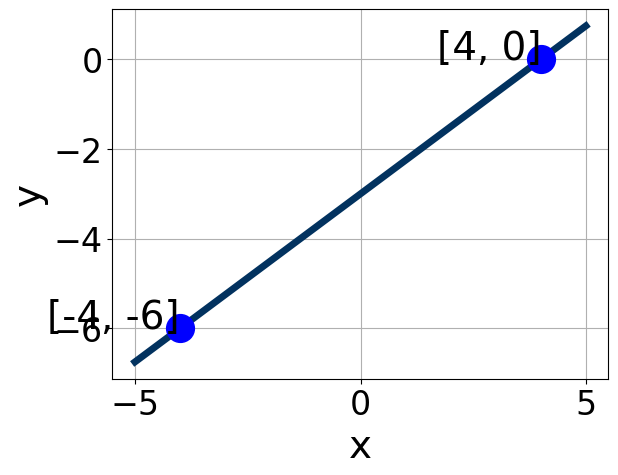
\includegraphics[width=0.5\textwidth]{../Figures/linearGraphToStandardCopyB.png}
\end{center}
\begin{enumerate}[label=\Alph*.]
\item \( A \in [0.6, 3.2], \hspace{3mm} B \in [-4.25, -3.33], \text{ and } \hspace{3mm} C \in [9, 16] \)
\item \( A \in [-3.3, -1.4], \hspace{3mm} B \in [2.39, 4.52], \text{ and } \hspace{3mm} C \in [-15, -9] \)
\item \( A \in [0.6, 3.2], \hspace{3mm} B \in [2.39, 4.52], \text{ and } \hspace{3mm} C \in [-15, -9] \)
\item \( A \in [-1.4, -0.2], \hspace{3mm} B \in [0.62, 1.44], \text{ and } \hspace{3mm} C \in [-5, 2] \)
\item \( A \in [-1.4, -0.2], \hspace{3mm} B \in [-1.04, -0.92], \text{ and } \hspace{3mm} C \in [0, 7] \)

\end{enumerate} }
\litem{
Write the equation of the line in the graph below in Standard form $Ax+By=C$. Then, choose the intervals that contain $A, B, \text{ and } C$.
\begin{center}
    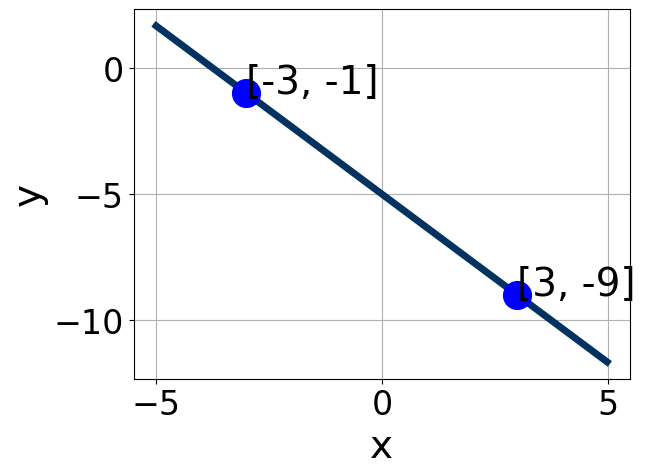
\includegraphics[width=0.5\textwidth]{../Figures/linearGraphToStandardB.png}
\end{center}
\begin{enumerate}[label=\Alph*.]
\item \( A \in [-2.4, 2.9], \hspace{3mm} B \in [-1.38, -0.75], \text{ and } \hspace{3mm} C \in [-7, 2] \)
\item \( A \in [3.1, 5.6], \hspace{3mm} B \in [-2.47, -1.52], \text{ and } \hspace{3mm} C \in [-7, 2] \)
\item \( A \in [-7.4, -2.2], \hspace{3mm} B \in [-2.47, -1.52], \text{ and } \hspace{3mm} C \in [-7, 2] \)
\item \( A \in [-2.4, 2.9], \hspace{3mm} B \in [0.03, 1.63], \text{ and } \hspace{3mm} C \in [-7, 2] \)
\item \( A \in [3.1, 5.6], \hspace{3mm} B \in [1.9, 2.74], \text{ and } \hspace{3mm} C \in [-7, 2] \)

\end{enumerate} }
\litem{
Solve the equation below. Then, choose the interval that contains the solution.\[ -13(-6x -17) = -3(8x -14) \]\begin{enumerate}[label=\Alph*.]
\item \( x \in [-2.2, -1] \)
\item \( x \in [1, 3.4] \)
\item \( x \in [-2.9, -2.2] \)
\item \( x \in [-6.8, -4.5] \)
\item \( \text{There are no real solutions.} \)

\end{enumerate} }
\litem{
Solve the linear equation below. Then, choose the interval that contains the solution.\[ \frac{-7x -5}{7} - \frac{-6x -5}{6} = \frac{3x + 7}{3} \]\begin{enumerate}[label=\Alph*.]
\item \( x \in [-2.5, -1.88] \)
\item \( x \in [-0.89, -0.03] \)
\item \( x \in [-7.11, -6.8] \)
\item \( x \in [-4.78, -3.63] \)
\item \( \text{There are no real solutions.} \)

\end{enumerate} }
\litem{
Solve the equation below. Then, choose the interval that contains the solution.\[ -7(9x + 15) = -13(19x + 8) \]\begin{enumerate}[label=\Alph*.]
\item \( x \in [-1.24, -0.95] \)
\item \( x \in [1, 1.2] \)
\item \( x \in [-0.08, 0.47] \)
\item \( x \in [-0.87, -0.28] \)
\item \( \text{There are no real solutions.} \)

\end{enumerate} }
\litem{
Solve the linear equation below. Then, choose the interval that contains the solution.\[ \frac{3x -9}{4} - \frac{-7x + 8}{5} = \frac{3x + 8}{3} \]\begin{enumerate}[label=\Alph*.]
\item \( x \in [5.6, 6.3] \)
\item \( x \in [1.9, 4.9] \)
\item \( x \in [21.3, 22.1] \)
\item \( x \in [-0.1, 2.1] \)
\item \( \text{There are no real solutions.} \)

\end{enumerate} }
\litem{
First, find the equation of the line containing the two points below. Then, write the equation as $ y=mx+b $ and choose the intervals that contain $m$ and $b$.\[ (-6, 6) \text{ and } (-8, -7) \]\begin{enumerate}[label=\Alph*.]
\item \( m \in [-8.5, -1.5] \hspace*{3mm} b \in [-60, -55] \)
\item \( m \in [3.5, 8.5] \hspace*{3mm} b \in [-2, 3] \)
\item \( m \in [3.5, 8.5] \hspace*{3mm} b \in [9, 18] \)
\item \( m \in [3.5, 8.5] \hspace*{3mm} b \in [40, 46] \)
\item \( m \in [3.5, 8.5] \hspace*{3mm} b \in [-51, -36] \)

\end{enumerate} }
\end{enumerate}

\end{document}